\chapter{Quantum walk simulator software}

In this chapter, I present the simulator software I wrote. I discuss the currently available solutions, why I chose to write the software, the architecture, the components and design patterns I used, the challenges I faced during the development and the solutions I found.

\section{Software design}

I developed the software using Python 3, based on the Strategy design pattern. It supports graphs commonly found in the literature while also providing a method for combining them, facilitating experimentation on several kinds of regular graphs. This composition is also the foundation of the quantum walk. It can simulate classical and quantum walks on the same graphs and produce a report file detailing the results. In the quantum case, the characteristics of the walk are also dependent on the type of coin used to generate the probabilities, which can be defined in several ways. The program includes the Hadamard, Grover, and Fourier coins and can easily be extended with others.

Running several simulations, I compared the behavior of classical and quantum walks and demonstrated the quantum characteristics expected from the theoretical literature, the ballistic nature of the Hadamard walk, and the cyclic property of quantum walks.

\subsection{Currently available solutions}

Since publicly accessible quantum computers currently only have around 5-10 qubits, it is not viable at the moment to run quantum walks on a real quantum computer. Hence why, when I started researching quantum walks, I quickly began looking into simulator software. While there are many of these currently available, most of them have at least one of the following issues:

\begin{enumerate}
\item Not maintained and developed anymore: the last commit was years ago.
\item Written in a low-level language, like C++, in a script-like fashion, with a prominent focus on memory and performance optimization while neglecting readability, modularity and extensibility.
\item Works exclusively on a specific type of graph, for example, $n$-dimensional lattices only.
\item Unable to compare and contrast classical and quantum walks on the same graph, running only quantum simulations.
\item Hard to understand as a novice.
\end{enumerate}

There is no general, open-source solution available that is designed and developed using sound software engineering practices and an architecture that allows for experimentation with different kinds of graphs with both classical and quantum simulations available.

I intend my solution to be valuable for research purposes while also providing a readable open-source codebase for college students to study the algorithm.

\subsection{Architecture}

The architecture of my simulator program employs the Strategy design pattern, which is described in the following way:

''Define a family of algorithms, encapsulate each one, and make them interchangeable. Strategy lets the algorithm vary independently from clients that use it.''~\cite{DesignPatterns}

\begin{figure}[H]
  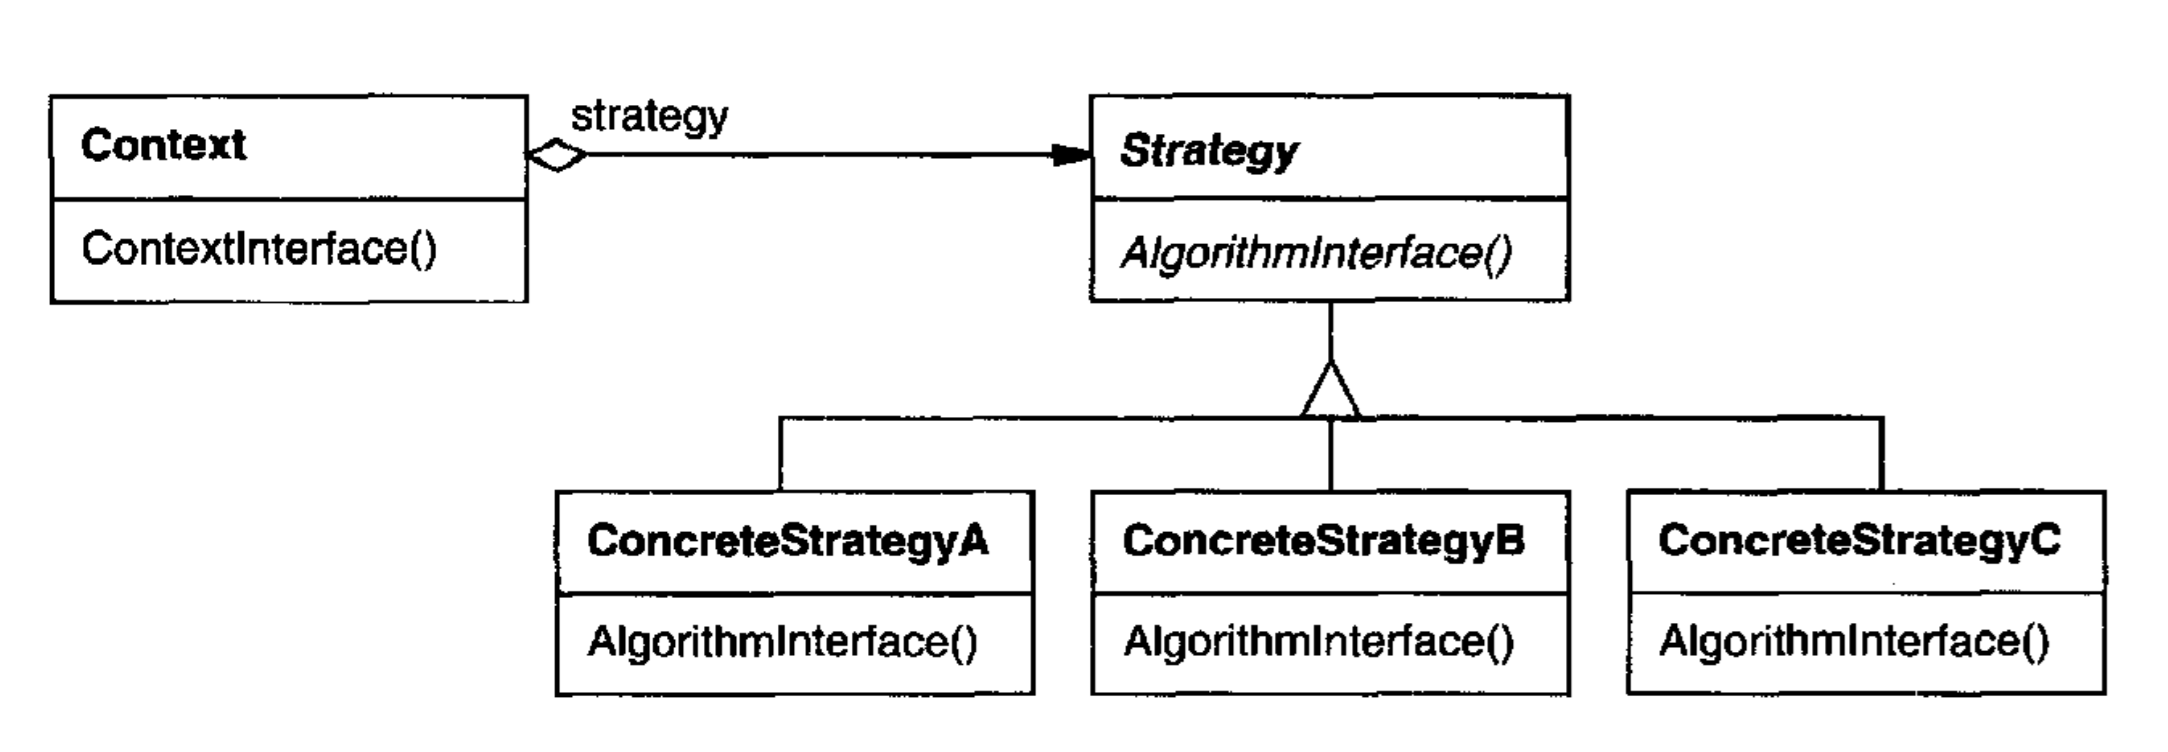
\includegraphics[width=\linewidth]{./figures/program/strategy.png}
  \caption{UML diagram for the Strategy design pattern from~\cite{DesignPatterns}}
\end{figure}

This is a great design pattern for research purposes since it facilitates experimentation with various algorithms for the same purpose. It also makes the code easily readable, as the Strategy interface provides an abstraction layer between the Context and the concrete implementation.

\subsection{Language choice}

With the specified goals and the architecture in mind, I needed a language that is object-oriented, easily readable by beginners and has extensive capabilities for using complex numbers, linear algebra and plotting. For these purposes, I choose the Python language. Python is concise, it reads like pseudocode and has libraries such as NumPy, SciPy and Matplotlib, and so on, covering all areas of data science. Furthermore, it is well-known and extensively used by researchers with no software engineering background, allowing for easier collaboration.

\subsection{High level design}

The source code of the software can be divided into three parts:

\begin{itemize}
    \item Graph models
    \item Simulators
    \item Running, configuration and result collection
\end{itemize}

\begin{figure}[H]
  
\includegraphics[width=\linewidth]{./figures/program/uml.png}
  \caption{UML diagram for the Graph models and Simulators}
\end{figure}

On the UML diagram above, the SubGraph class is a Strategy, with the following ConcreteStrategy implementations:

\begin{itemize}
    \item BinaryTree
    \item Bipartite
    \item Circle
    \item Grid
    \item Hypercube
    \item Path
    \item Random
\end{itemize}

Each of these employs an oracle that calculates neighbouring vertices on-the-fly.

Furthermore, the Simulator is also a Strategy, implemented by the Classical and the Quantum classes, the latter using the Coin Strategy, implemented by the Hadamard, Grover and Fourier (DFT) classes.

(For a cleaner diagram, I did not picture the SubGraph and Coin implementations.)

\subsection{Graph models}

I ran several experiments on various graphs while researching quantum graph walks, including paths, circles, bipartite graphs, hypercubes, and grids. Initially, I directly generated and stored their adjacency matrices, however, I quickly ran into memory scaling issues with this approach. Furthermore, in quantum research, graphs are typically built like 'Legos', glueing together a few common types, which was challenging to do with my original approach.

To combat these issues, I switched from the adjacency matrix representation to the oracle representation. The oracle is a function that returns the neighbours of a given vertex. Since I was using common graphs, I could calculate neighbouring indexes on-the-fly without storing anything about these graphs and only querying what is needed at the current step, dramatically reducing the memory requirements of the graph models.

\subsection{Simulators}

I implemented a classical and a quantum simulator class. The quantum simulator can currently simulate directed $k$ regular graphs, however since the permutation matrix decomposition, or in the undirected case, the edge coloring of the matrix is an NP-complete problem, in the current setup, the graph oracle must be implemented in a way that returns the neighbours in the same color order for all inputs. Since the human programmer designs the oracle, this is not a critical limitation at the moment. I have implemented a check as a safety guard to ensure the resulting shift matrices are unitary in case an error is made while coding one of the oracles.

\subsection{Running, configuration and result collection}

Using the above classes, I developed a framework in which experimental runs can be configured very quickly. The results of the run are collected in an aggregated Latex document, using Matplotlib for creating various graphics. It contains the given graph, the named type of the subgraphs, the adjacency matrices, the distribution results of the simulations, including empirical hitting and mixing times and the eigenvalues and eigenvectors of the evolution operators. In the following chapter, I present several examples collected from these Latex reports of my experiments.

\subsection{Availability}

My simulator software is available under the open-source MIT license on my personal Github account, under the following link:

\url{https://github.com/nemkin/quantum}